%%%%%%%%%%%%%%%%%%%%%%%%%%%%%%%%%%%%%%%%%%%%%%%%%%%%%%%%%%%%%%%%%%%%%%%%
%    INSTITUTE OF PHYSICS PUBLISHING                                   %
%                                                                      %
%   `Preparing an article for publication in an Institute of Physics   %
%    Publishing journal using LaTeX'                                   %
%                                                                      %
%    LaTeX source code `ioplau2e.tex' used to generate `author         %
%    guidelines', the documentation explaining and demonstrating use   %
%    of the Institute of Physics Publishing LaTeX preprint files       %
%    `iopart.cls, iopart12.clo and iopart10.clo'.                      %
%                                                                      %
%    `ioplau2e.tex' itself uses LaTeX with `iopart.cls'                %
%                                                                      %
%%%%%%%%%%%%%%%%%%%%%%%%%%%%%%%%%%
%
%
% First we have a character check
%
% ! exclamation mark    " double quote  
% # hash                ` opening quote (grave)
% & ampersand           ' closing quote (acute)
% $ dollar              % percent       
% ( open parenthesis    ) close paren.  
% - hyphen              = equals sign
% | vertical bar        ~ tilde         
% @ at sign             _ underscore
% { open curly brace    } close curly   
% [ open square         ] close square bracket
% + plus sign           ; semi-colon    
% * asterisk            : colon
% < open angle bracket  > close angle   
% , comma               . full stop
% ? question mark       / forward slash 
% \ backslash           ^ circumflex
%
% ABCDEFGHIJKLMNOPQRSTUVWXYZ 
% abcdefghijklmnopqrstuvwxyz 
% 1234567890
%
%%%%%%%%%%%%%%%%%%%%%%%%%%%%%%%%%%%%%%%%%%%%%%%%%%%%%%%%%%%%%%%%%%%
%
%    J.-L. Ley
%
\documentclass[12pt]{iopart}
\newcommand{\gguide}{{\it Preparing graphics for IOP journals}}
%Uncomment next line if AMS fonts required
%\usepackage{iopams}  
\usepackage[english]{babel}
% \usepackage[latin1]{inputenc}
\usepackage[T1]{fontenc}	% accent dans le pdf
%\usepackage[utf8x]{inputenc}
\usepackage{colortbl}

\usepackage{caption}
\usepackage{tabularx} % Pour avoir des tableaux d'une largeur bien d�finie
\usepackage{graphicx} 
\usepackage{amsfonts}
 \usepackage[squaren,Gray,cdot]{SIunits} % pour avoir de jolies unit�s
 \usepackage{subfig} % Pour avoir des sous-figures.
\usepackage{multirow}
\usepackage{lscape}
\usepackage{pdflscape}
\usepackage{footnote}
%\usepackage{amsmath}



\begin{document}

\title{Monitoring Ion Therapy with a Compton Camera: Simulation Studies of the Clinical Feasibility}

\author{J.-L.~Ley$^1$, D.~Dauvergne$^3$, N.~Freud$^2$, J.~Krimmer$^1$, J.~M.~Létang$^2$, V.~Maxim$^2$, M.-H.~Richard$^1$, and \'E.~Testa$^1$}

\address{$^1$Univ Lyon, Université Claude Bernard Lyon 1, CNRS/IN2P3, Institut de Physique Nucléaire de Lyon, 69622 Villeurbanne, France}
\address{$^2$Univ Lyon, INSA-Lyon, Université Claude Bernard Lyon 1, UJM-Saint Étienne, CNRS, Inserm, Centre Léon Bérard, CREATIS UMR 5220 U1206, F-69373, Lyon, France}
\address{$^3$LPSC, Université Grenoble-Alpes, CNRS/IN2P3 UMR5821, F-38026 Grenoble, France}
\ead{jeanluc.ley@gmail.com}

\begin{abstract}
The aim of irradiation monitoring during a treatment in ion therapy is to control in real time the agreement between the delivered dose and the planned treatment. In fact, the discrepancies might come from uncertainties such as the planning accuracy by itself, or by variations due to the positioning or the anatomical changes of the patient. This can lead to ion-range variations of a few millimeters. Several devices are under development over the world to detect secondary radiation, which are correlated to the dose deposited by incident ions [1]. Compton cameras are in particular investigated for their potential high efficiency to detect prompt-gammas [2-5]. The present work aims at discussing the clinical applicability of a Compton camera design by means of Monte Carlo simulations validated against measurements of single and coincidence rates.

\end{abstract}


%Uncomment for PACS numbers title message
%\pacs{00.00, 20.00, 42.10}
% Uncomment for Submitted to journal title message
\submitto{\PMB}
% Keywords required only for MST, PB, PMB, PM, JOA, JOB? 
\vspace{2pc}
\noindent{\it Keywords}: Compton Camera, ion therapy, clinical applicability
% Comment out if separate title page not required
\maketitle
%
\newpage

\tableofcontents


\section{Introduction}

%%%----------------------------------------------------------------------
%%%----------------------------------------------------------------------
%%%------------- Materials and methods    -----------------------------------
%%%----------------------------------------------------------------------
%%%----------------------------------------------------------------------

\section{Material and methods}

\subsection{Simulation setup\newline}

The simulation consists of the irradiation of a patient by an ion beam and the detection of the secondary particles emitted by means of the Compton camera prototype. The patient is replaced by a cylindrical PMMA\footnotemark[1] phantom of 15 centimeters diameter and 20 centimeters length. The Compton camera prototype is composed of a scatterer, an absorber and a scintillating fiber hodoscope. The mechanical structures of the detectors, the scatterer's strips and the hodoscope are not modelled in this study. The scatterer is a stack of seven layers of double-sided silicon strip detectors (DSSD) of 90 $\times$ 90 $\times$ 2 $\rm{mm}^3$ with 64 strips on each side. The absorber consists of 96 blocks of streaked BGO\footnotemark[2] crystals of 38 $\times$ 38 $\times$ 30 $\rm{mm}^3$. . Moreover, the absorber is modelled by a monoblock of BGO crystal of 380 $\times$ 380 $\times$ 30 $\rm{mm}^3$ equivalent to 100 single blocks. The distance between the camera and the center of the PMMA phantom is set at 20 centimeters in order to fit with a realistic distance to the patient. The distance between each silicon layer is one centimeter and the distance from the last silicon layer to the absorber is 40 centimeters. The distance between the stack of silicon layers and the absorber is a compromise between the camera efficiency and the discrimination by time of flight measurement. The setup is described figure \ref{fig:fig_setup_CC_simulation_Hadronth}.\newline

	\begin{figure} [!hbtp]	
	\centering
	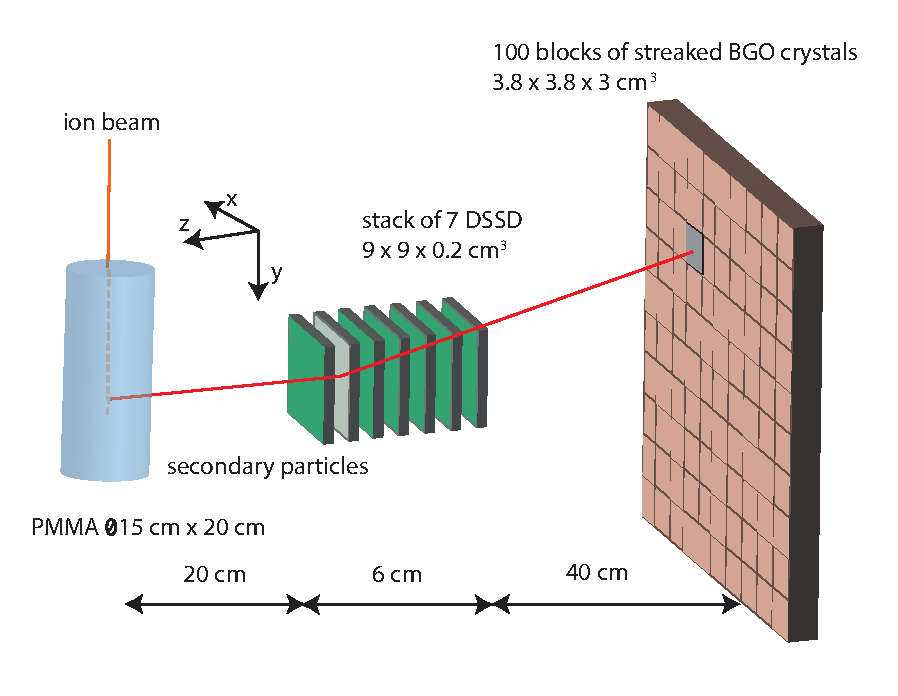
\includegraphics[width=0.7\textwidth]{./Figure/Material_Methods/Compton_Camera_hadontherapy_PMMA_Cylinder_EN.eps}
		\caption{Modelling of the patient (PMMA cylinder) and the Compton camera prototype. This configuration is used for all the results presented in this paper.}
	\label{fig:fig_setup_CC_simulation_Hadronth}
	\end{figure}

 \footnotetext[1]{PolyMethylMethAcrylate}
\footnotetext[2]{Bismuth Germanate} 

\subsection{Hadronic models used in Geant4\newline}

The study is based on the Monte Carlo methods with the Geant4 toolkit, version 9.6 patch 02. Geant4 has been developed by the CERN for the high energy physics experiments. It was shown that it could also be used in ion therapy studies \cite{cirrone_hadrontherapy_2011,toshito_new_2010}. However, some improvements remains to do in order to adjust the hadronic models \cite{dedes_assessment_2014} .
The interaction processes in the matter are described by means of different models according to the type of particles. A resume of those different models is given table \ref{table:table_modele_physic_CC_simulation_Hadronth}. Additionally, the Doppler broadening and the polarization is taking into account. 

\definecolor{Gray}{gray}{0.9}

\begin{table}[ht]
\label{physlist_ion}
\caption{Hadronic models used in the simulations Geant4.}
\begin{scriptsize}
\begin{center}
\renewcommand{\arraystretch}{1.2}
%\begin{tabular} {>{\columncolor[gray]{0.9}}cccc}\hline  
\begin{tabular} {cccc}\hline
%\rowcolor{Gray}
\textbf{Processus} & \textbf{Protons} & \textbf{Ions} & \textbf{Neutrons} \\ \hline 
\textbf{Electromagnetic} & \multicolumn{3}{c}{standard$_{\rm{option3}}$} \\ %\hline
\textbf{Inelastic} & G4BinaryCascade & G4QMDReaction  &  G4BinaryCascade  \\ 
 & & (G4IonsShenCrossSection)&+ G4NeutronHPInelastic ($<$19 MeV)\\ %\hline
\textbf{Elastic} & G4LElastic & G4LElastic & G4LElastic + G4NeutronHPElastic ($<$19 MeV)\\ %\hline
\textbf{Fission} & / & / & G4LFission + G4NeutronHPFission($<$19 MeV) \\ %\hline
\textbf{Capture} & / & / & G4LCapture +  G4NeutronHPCapture ($<$19 MeV) \\ %\hline
\textbf{Radioactivedecay} & / & G4Radioactivedecay & / \\ \hline
\end{tabular}
\end{center}
\end{scriptsize}
\label{table:table_modele_physic_CC_simulation_Hadronth}
\end{table}

\subsection{Particles of interest}
\label{subsection:Particules_Etudiees_CC_hadrontherapy_Geant4}

We study the two main particles used in clinics, namely the protons and the carbon ions. The ion range of interest is 15.2 cm in the PMMA target. The energy associated with the range is 160 MeV for the protons and 305 MeV/n for the carbon ions. The beam delivered during a real treatment has a Gaussian profile at the enter of the patient. The standard deviation for a proton beam is 5 mm at 160 MeV and 3.5 mm for a carbon ion beam at 305 MeV/n. The modelling of the Compton camera does not change with the type of incident particles. The statistic for a spot in pencil beam scanning (PBS) mode for protons is $10^8$ particles and $10^5$ particles for carbon ions. The beam time structure is applied during the post treatment.\newline


\subsection{Data treatment}
\label{subsection:Treatment_data_CC_hadrontherapy_Geant4}

\subsubsection{Detector resolutions\newline}
\label{subsubsection:Resolution_detector_CC_hadrontherapy_Geant4}

The Monte Carlo simulation parameters are as close to reality as possible in order to get relevant results. The detector resolutions play an important role in the Compton camera performances. The absorber's spatial resolution influences the position of the apex of the Compton cone and influences its axis orientation. The energy resolution has effect on the  Compton cone aperture angle and the timing resolution impacts the coincidence windows between the absorber and the scatterer. The hodoscope is not included in the simulation but its timing resolution is taking into account for the time of flight discrimination. The detector resolutions are modelled in relation to the resolutions measured or estimated for each detector. The spatial resolution, the energy resolution and the timing resolution are presented in the table \ref{table:table_resolution_detecteurs_CC_simulation_Hadronth}.

\begin{table} [!htbp]
\centering
%\begin{tabular}{>{\columncolor[gray]{0.9}}ccc}
\caption{Realistic resolutions applied during the simulations.}
\begin{tabular}{cccc}
\hline
\textbf{Resolution (FWHM) at 1 MeV} & \textbf{Scatterer} & \textbf{Absorber} &\textbf{Hodoscope}\\
\hline 
\textbf{spatial [mm]	}			 &     0.9		 &  5	 			&   /	\\
%\hline
\textbf{energy [\%]}				&	2.3		&  17				&   /     \\
%\hline
\textbf{timing [ns]}	        			&	15		&	3 			&  1     \\
\hline
\end{tabular}
\label{table:table_resolution_detecteurs_CC_simulation_Hadronth}
\end{table}

\subsubsection{Modelling of the ion beam structure\newline}
\label{subsubsection:modelisation_fasceau_ions_CC_hadrontherapy_Geant4}
 


The beam time structure should have a direct impact on the Compton camera capacities to detect a particle in coincidence between the scatterer and the absorber.
Two beam time structures have been modelled: one of IBA cyclotron C230 for protons (used in 16 clinical centers worldwide) and one of synchrotron installed at the Heidelberg Ion Therapy Center (HIT) in Germany for carbon ions. Depending on the ion energy and the beam intensity, the beam microstructure will change. We are focusing in this study to the microstructure at a specific energy and also at the influence of the variation of the intensity. In the case of protons at 160 MeV, the ions are grouped in bunches of 2 ns at a frequency of 106 MHz (9.42 ns) \cite{f_roellinghoff_real-time_2014}. The clinical beam intensity is 3.2 nA which corresponds to about 200 protons per bunch. Concerning the carbon ion beam at 305 MeV/u, the estimated microstructure is a bunch of 30 ns at a frequency of 5.9 MHz (170 ns). The clinical beam intensity for carbon ions is $5\times10^7$ ions/s which corresponds to about 9 ions per bunch. This beam structure is extrapolated from measurements done by our team in 2013 at HIT. The time beam structure was measured for 200 MeV/u and 400 MeV/u carbon ion beams with a two scintillating fiber hodoscope and the spill signal given by the accelerator. The figure \ref{fig:fig_structure_temps_faisceau_HIT_2013_CC_simulation_Hadronth} shows the beam structure for carbon ions at 400 MeV/u. The pulses have a spill period of 150.2 ns and a bunch is 21.5 ns. A dedicated measure should be done for the energy of interest for this study (305 MeV/u).\newline
Moreover, the measurements have shown that the spill phase change during the extraction which involves  the HF signal from the synchrotron can not be used to locate the pulses. The use of the hodoscope seems required.\newline

	\begin{figure} [!hbtp]	
	\centering
	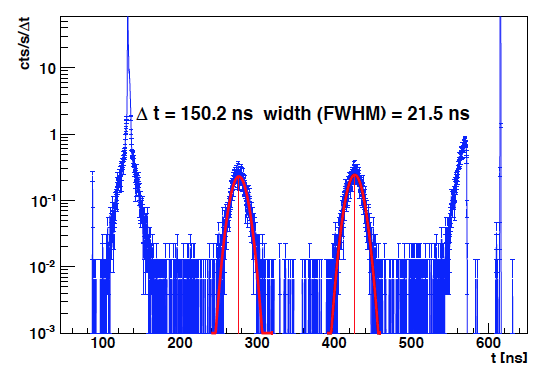
\includegraphics[width=0.5\textwidth]{./Figure/Material_Methods/2013_Structure_Time_Beam_400MeV.png}
	\caption{Time structure measured from a carbon ion beam at 400 MeV/u delivered at HIT. The pulses have an extraction period of 150.2 ns and the bunches are 21.5 ns FWHM. The measure was done with a two scintillating fiber hodoscope.}
	\label{fig:fig_structure_temps_faisceau_HIT_2013_CC_simulation_Hadronth}
	\end{figure}


Concerning the coincidence between the scatterer and the absorber, we allow a time window of 40 ns around an absorber event. It means that for an event detected in the absorber, it will be flagged as a coincidence if an event (corresponding to a deposit energy) in one the scatterer layers is detected in a window of -20 ns and + 20 ns around the absorber event. This coincidence windows is defined regarding of the silicon timing resolution which is 15 ns at the full width at half maximum. The table \ref{table:definition_beam_structure_CC_hadrontherapy_Geant4} resumes those characteristics for specific ions.

\begin{table} [!htbp]
\footnotesize
\centering
\caption{Beam structure applied to the simulation data.}
\setlength{\tabcolsep}{2pt}
%\hspace{-2.1cm}
\begin{tabular}{c>{\columncolor[gray]{0.9}}ccc}
\cline{2-4}
%\hline
		\multicolumn{2}{c}{ }		 & 					\textbf{Protons} & \textbf{Carbon ions}\\ 
%\hline
\cline{2-4}%\hline
\multirow{3}{*}\textbf{Clinical characteristics}		&	\textbf{Facility}	& IBA Cyclotron C230&   Synchrotron at HIT\\
											& \textbf{Clinical intensity}& $  2\times10^{10}$ p/s  & $  5\times10^{7}$ ions/s\\
											& \textbf{Energy} 			&160 MeV 			&    305 MeV/u\\
\cline{2-4}%\hline
\multirow{3}{*}\textbf{Beam structure}		&	\textbf{Bunch time [ns]}			& 3.2				&  30\\
											& \textbf{Period [ns]}		&   9.4 				& 170\\
											& \textbf{Particles/bunch} 	&217 			& 9\\
\cline{2-4}%\hline
\multirow{2}{*}\textbf{Detectors}						& \textbf{Coincidence window [ns]}		& 40 	&  40 \\
											&\textbf{Timing resolution [ns]} & \multicolumn{2}{c}{Si: 15 and BGO: 3}\\
\cline{2-4}%\hline
\end{tabular}
\label{table:definition_beam_structure_CC_hadrontherapy_Geant4}
\end{table}



\newpage
%---------------------------------------------------------------
%---------------------------------------------------------------
\subsubsection{Coincidence\newline}
\label{subsubsection:definition_beam_structure_CC_hadrontherapy_Geant4}

The Compton camera is based on a double interaction inside the scatterer and the absorber. A coincidence is defined as one energy deposit in the scatterer and one energy deposit in the absorber in a coincidence time windows given. A number of coincidence will be considered as background: quasi-simultaneous interaction from two secondary particles or a double interaction from the same particle different from a gamma.\newline
If a coincidence is detected but the two particles are not coming from the same incident ion, the coincidence is named fortuitous.
Otherwise, if a single particle from the same incident ion leaves energy in the absorber and the scatterer, the coincidence is named true.\newline
It can be distinguish two types of true coincidence: a single gamma ray, which is a true gamma, and the rest of possibilities (electron, proton, neutron) which is background. The coincidences of interest are the true gamma. 

The figure \ref{fig:fig_explication_coincidence_CC_simulation_Hadronth} resumes the different definitions of coincidendes in the Compton camera.
	\begin{figure} [!hbtp]	
	\centering
	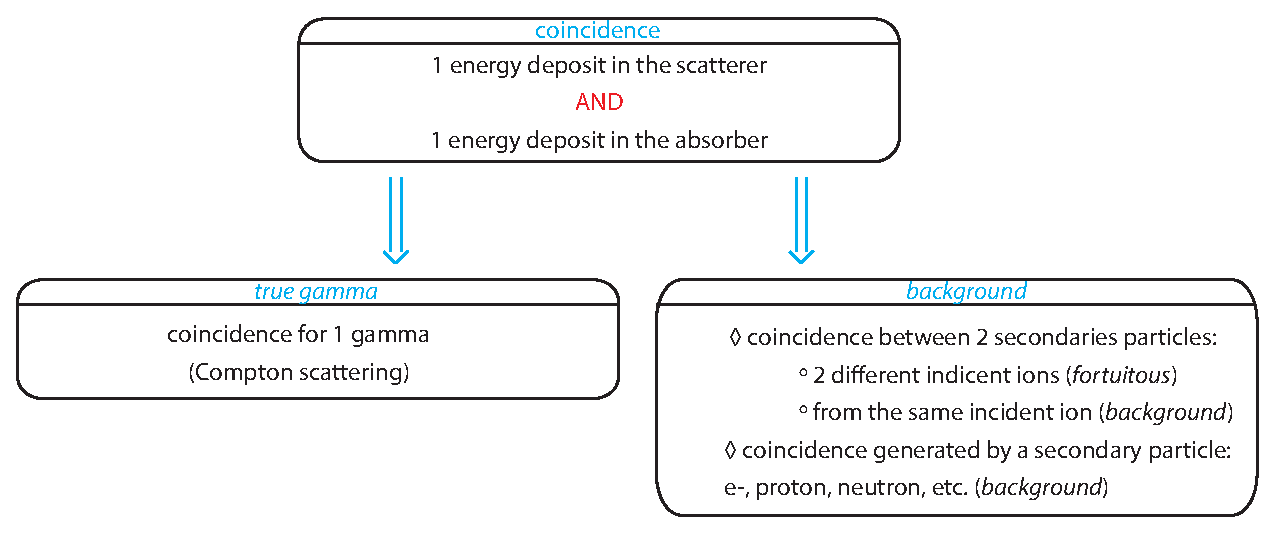
\includegraphics[width=0.9\textwidth]{./Figure/Material_Methods/Schema_coincidence_EN.eps}
	\caption{Diagram showing the different definitions of coincidendes in the Compton camera.}
	 \label{fig:fig_explication_coincidence_CC_simulation_Hadronth}
	\end{figure}


\subsubsection{Time of flight discrimination and energy cuts\newline}

\textit{Time of flight (TOF) information}\newline

The goal is to eliminate the massive or charged particles (proton, electron, neutron) creating a coincidence in the Compton camera thanks to their speed. In fact, the photons are moving at the light speed when the other particles are moving slower due to their mass. To discriminate the particles with their speed, the time information coming from the hodoscope and the time information coming from the absorber are used. The difference between that information is named time of flight (equation 1). However, the hodoscope is not modelling in this study. As the Monte Carlo code consists to follow all stories individually, the time between the incident particle's creation and the secondary particle detection in the absorber is considered as the time of flight. Moreover, the hodoscope has a timing resolution about one nanosecond at full width at half maximum, so it is taking into account in the TOF estimation.

\begin{eqnarray*}
TOF_{theoretical} = t_{absorber}-t_{hodoscope}\\
TOF_{simulation} = t_{absorber}+t_{creation} + u_{hodoscope}
\end{eqnarray*}
With $u_{hodoscope}$  the hodoscope resolution modelled by a Gaussian with a sigma of 1/2.35 ns. 

The time of flight spectrum resulting from the simulation shows that the coincidences of interest are included in a window between 0 and 6 ns (figure \ref{fig:fig_TOF_distribution_CC_simulation_Hadronth}). Therefore, all the coincidences with a TOF higher than 6 ns will be excluded from the results. 

	\begin{figure} [!hbtp]	
	\centering
	\caption{Time of flight spectrum obtained by means of the simulation and for a proton beam.}	
	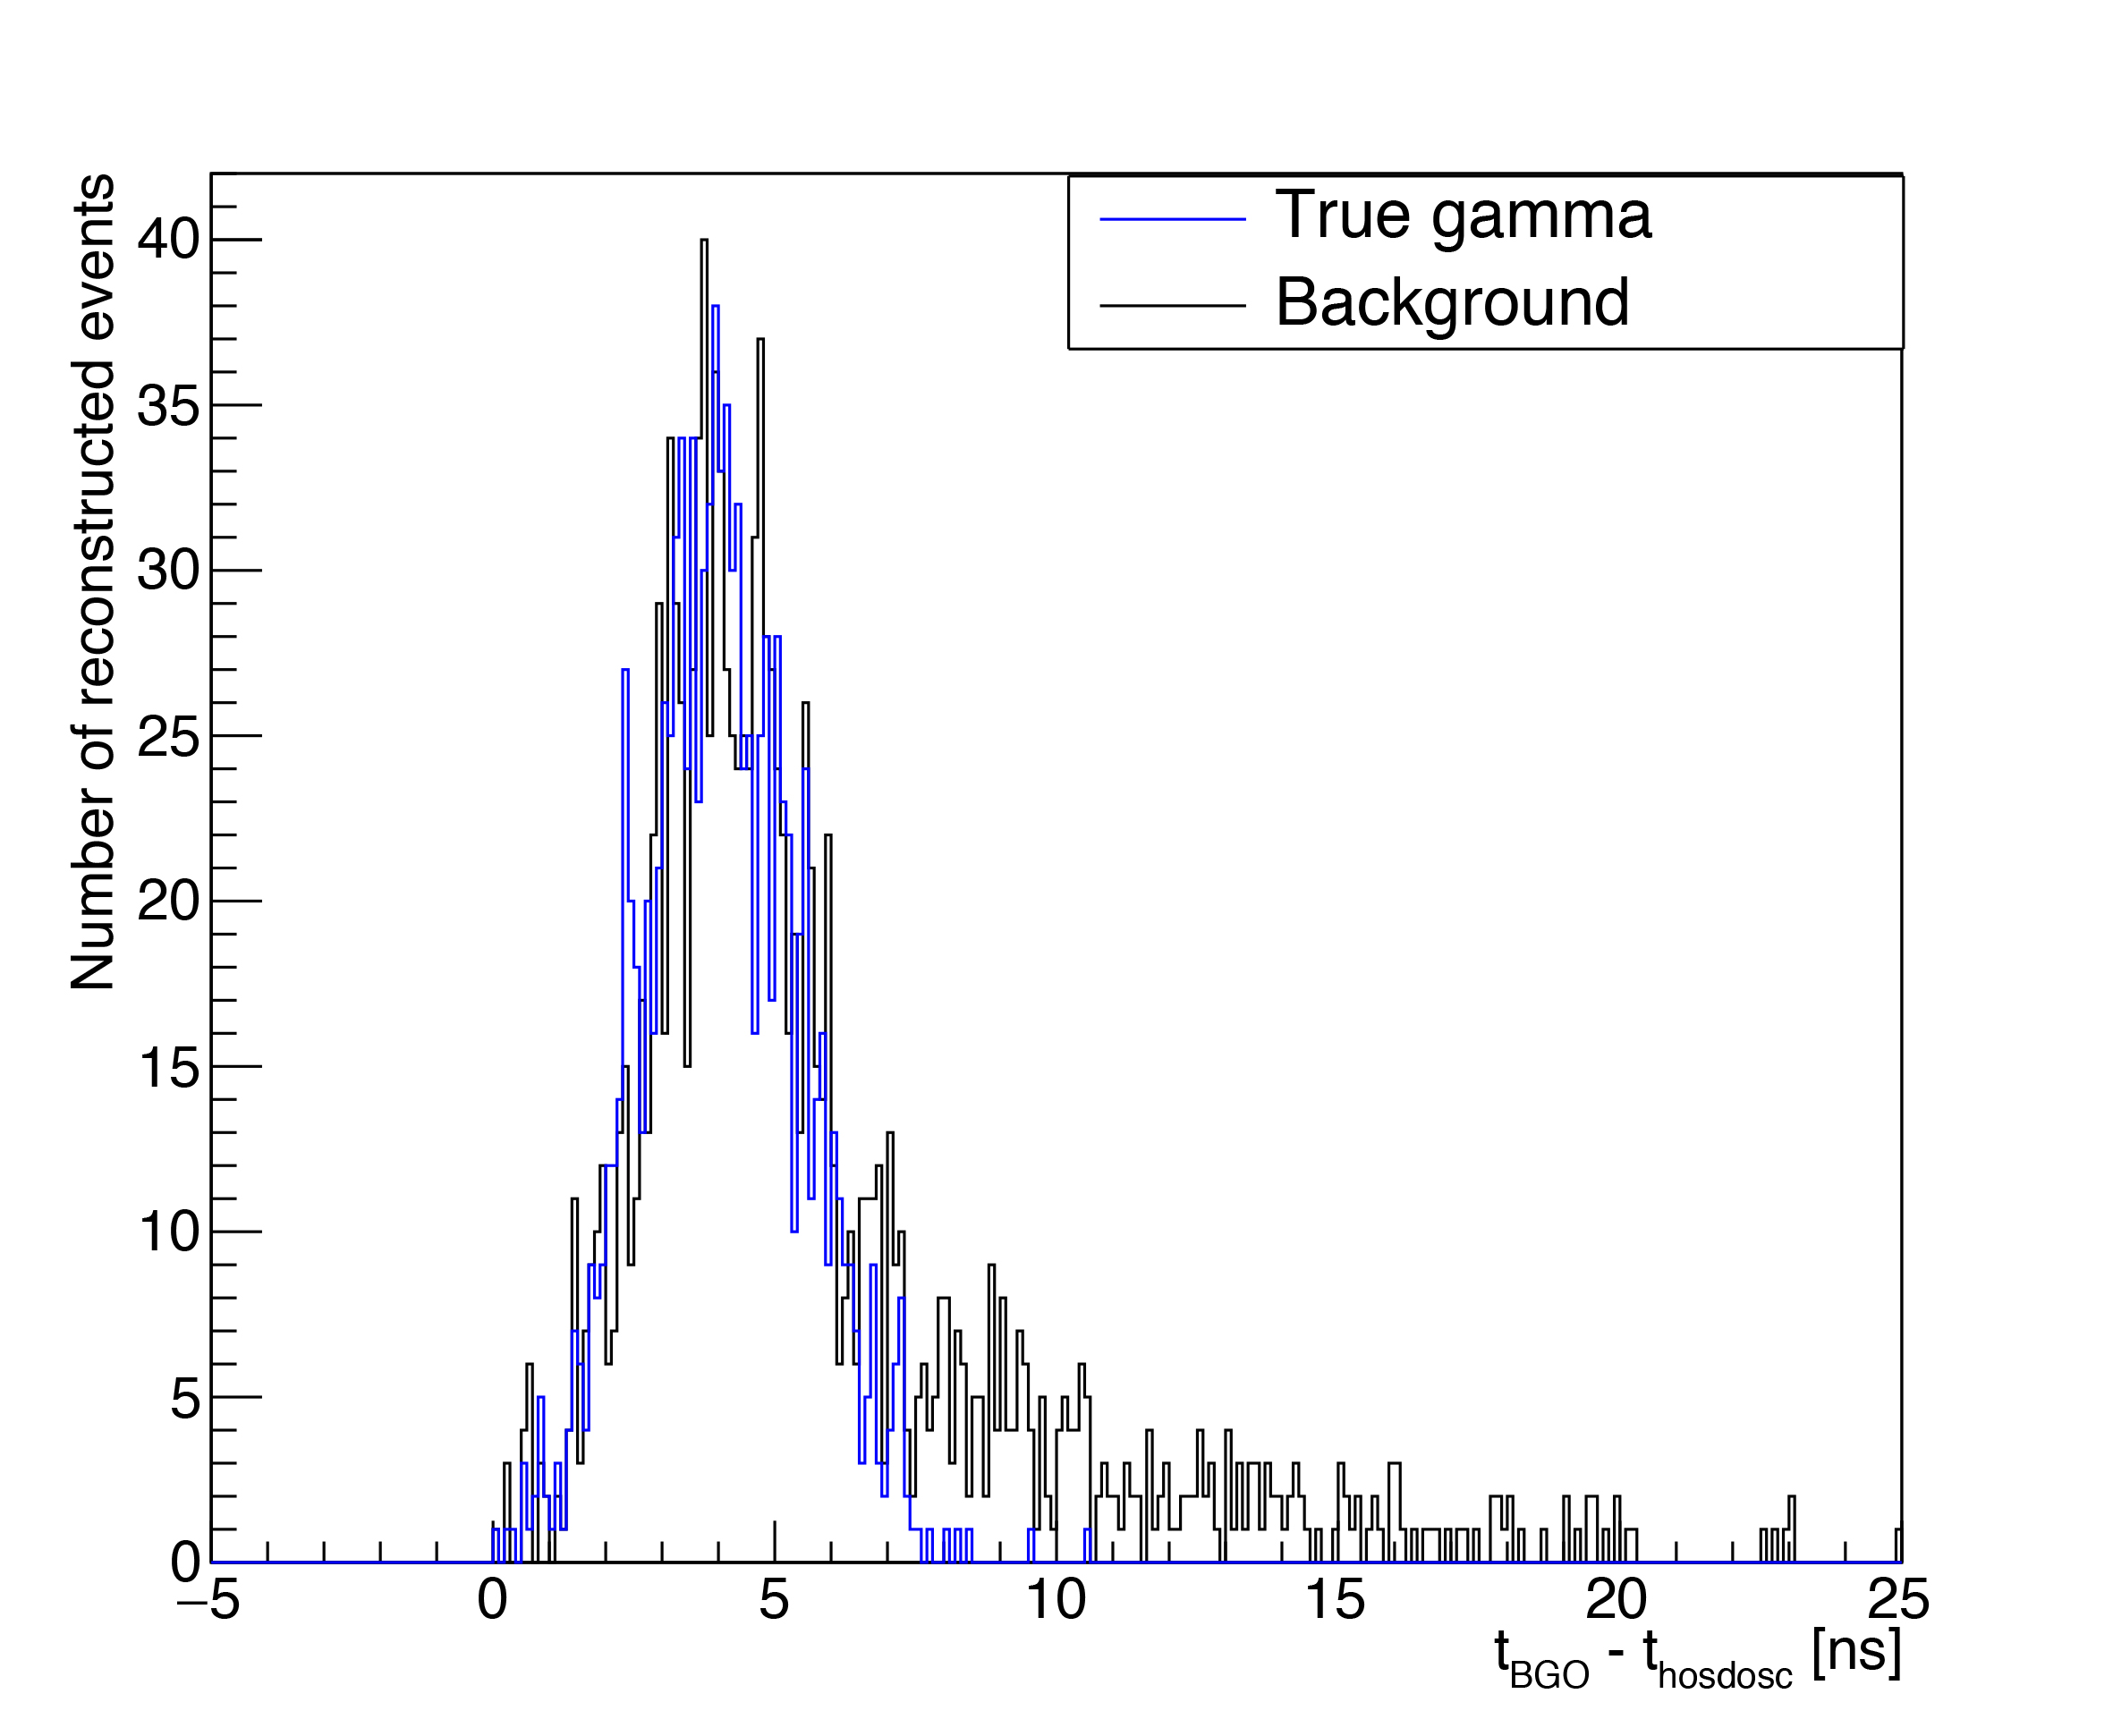
\includegraphics[width=0.6\textwidth]{./Figure/Material_Methods/2015_01_04_TOF_spectra_NoCut_1Proton_ResolTemporelle_applied_these.jpg}
	\label{fig:fig_TOF_distribution_CC_simulation_Hadronth}
	\end{figure}

\textit{Energy cuts}\newline

Energy triggers are also defined for the detectors: 50 keV for the silicon layers and 100 keV for the absorber. An additional energy cut is practiced to the total energy absorbed in the camera and it is set at 1 MeV. In fact, the main gamma rays of interest have an energy upper at 1 MeV.

\subsection{Reconstruction algorithm}

\subsubsection{Line-cone algorithm\newline}
A simple method is used to reconstruct the emission position of the events detect in coincidence: the reconstruction line-cone. Thanks to the deposited energies in the detectors and the interaction positions, a cone is calculated which contains the event emission point. The energies enable to calculate the aperture of the Compton cone by way of the following equation:

\begin{equation}
cos(\theta_{Compton}) = 1-m_ec^2\left(\frac{1}{E_{absorber}}-\frac{1}{E_{initial}}\right)
\end{equation}

	
With $E_{initial} = E_{absorber} + E_{silicon}$\newline
$E_{absorber}$ the energy deposited in the absorber and $E_{silicon}$ the energy deposited in the scatterer.\newline

We assume that the initial energy of the gamma ray is fully absorbed in the absorber. This hypothesis combined to the detector energy resolutions lead to a potential uncertainty on the cone aperture. The interaction position in the scatter gives the cone apex and the position in the absorber gives the cone axis. The intersection of all the reconstructed cones gives the emission source point. In order to simplify the reconstruction and limit the possibilities, the beam direction is used to obtain just two solutions: the beam direction intersects the cone in two points. Only one of those solutions is the good one and the other will give a wrong information. As the original position is unknown when the gamma ray is detected in coincidence, the results presented in the next section take into account the two solutions.\newline

\subsubsection{LM-MLEM algorithm\newline}	

The iterative method allows to get a 3D image and allows to take into account the spatial resolution and the energy resolution of the detectors. Few iterative algorithms have been developed for the hadrontherapy  \cite{schone_common_2010, zoglauer_design_2011,gillam_compton_2011,mackin_evaluation_2012,lojacono_low_2013}.

The iterative algorithm  \textit{List-Mode Maximum Likelihood Expectation Maximization} (LM-MLEM) is a MLEM version which allows to free from sinograms and to reconstruct the image directly from the list of events detected. \newline
The objective is to find the emission point of the gamma ray which produces the coincidence detected in the Compton Camera. 
The first step is to define the volume which includes the origin of the prompt gamma ray detected. This volume is divided in equal voxels and the emission intensity is assumed homogeneous for each voxel $j$ and follows a Poisson distribution of parameter $\lambda_j$. The vector contains the emissions intensities of all the voxels and the algorithm has to work it out. The system matrix $T$ is composed of the coefficients  $t_{ij}$ which represents the probability that a photon produce by the voxel $j$ is detected as a coincidence $i$ by the Compton camera. The probability for a gamma detected in coincidence to be emitted by the voxel $j$ is $s_j$.
The LM-MLEM algorithm starts with an initial value $\lambda^{(0)}$, which can be the simple backprojection.
The algorithm iterations are given by the following recurrence relation:

\begin{equation}
\lambda_j^{(l+1)} =  \frac{\lambda_j^{(l)} }{s_j} \sum\limits_{i=1}^{N_{\gamma}} t_{ij} \frac{1}{P_i^{(l)}},\quad \rm{avec}\quad  P_i^{(l)}=\sum\limits_{k=1}^{N_{v}} t_{ij}\lambda_k^{(l)},
 \label{eq:equation_lambda_compton_med_nucleaire}\newline
\end{equation}
where $N_{\gamma}$ is the number of detected events and $N_v$ is the number of voxels in the image.\newline

The LM-MLEM algorithm uses for this study is the one developed by the labortarory CREATIS in Lyon \cite{maxim_analytical_2009,lojacono_low_2013,maxim_filtered_2014,hilaire_compton_2014}.\newline
For each photon detected, the matrix $T$ is calculated by taking into account the uncertainties on the angle between the source and the scatterer and the angle between the scatterer and the absorber.
The matrix elements  $t_{ij}$  are calculated by:
\begin{equation}
 t_{ij} = K(\beta_i,E_{tot})\frac{|\rm{cos}(\theta_{\overrightarrow{V2V1})} |}{V_2V_1^2} \int\limits_{M\in v_j} \frac{|\rm{cos}(\theta_{\overrightarrow{V_1M})}| }{V_1M^2} h_i(M)dv,
 \label{eq:equation_tij_compton_med_nucleaire}\newline
\end{equation}
where $\beta_i$ is the Compton scattering angle, $V_1$ the interaction position in the scatterer, $V_2$ the interaction position in the absorber, $h_i$ the spatial kernel which models the uncertainties on the Compton angle for each voxel $M$, $K(\beta_i,E_{tot})$ the differential cross section and $v$ the reconstructed volume.\newline

In order to simplify and speed up the work out of the $t_{ij}$ matrix, the voxels located far from the cone are set to 0. The distance between the cone and the voxel is calculated for the center of the voxel. The spatial resolutions are not considered for the algorithm.\newline
The images are finally created from the matrix T thanks to Matlab software.

\subsection{Precision estimation\newline}


	
\newpage
	

\section{Results}

\subsection{CC efficiency\newline}

	\begin{figure} [!hbtp]	
	\centering
	\caption{Detection efficiency function of the Compton Camera position.}	
	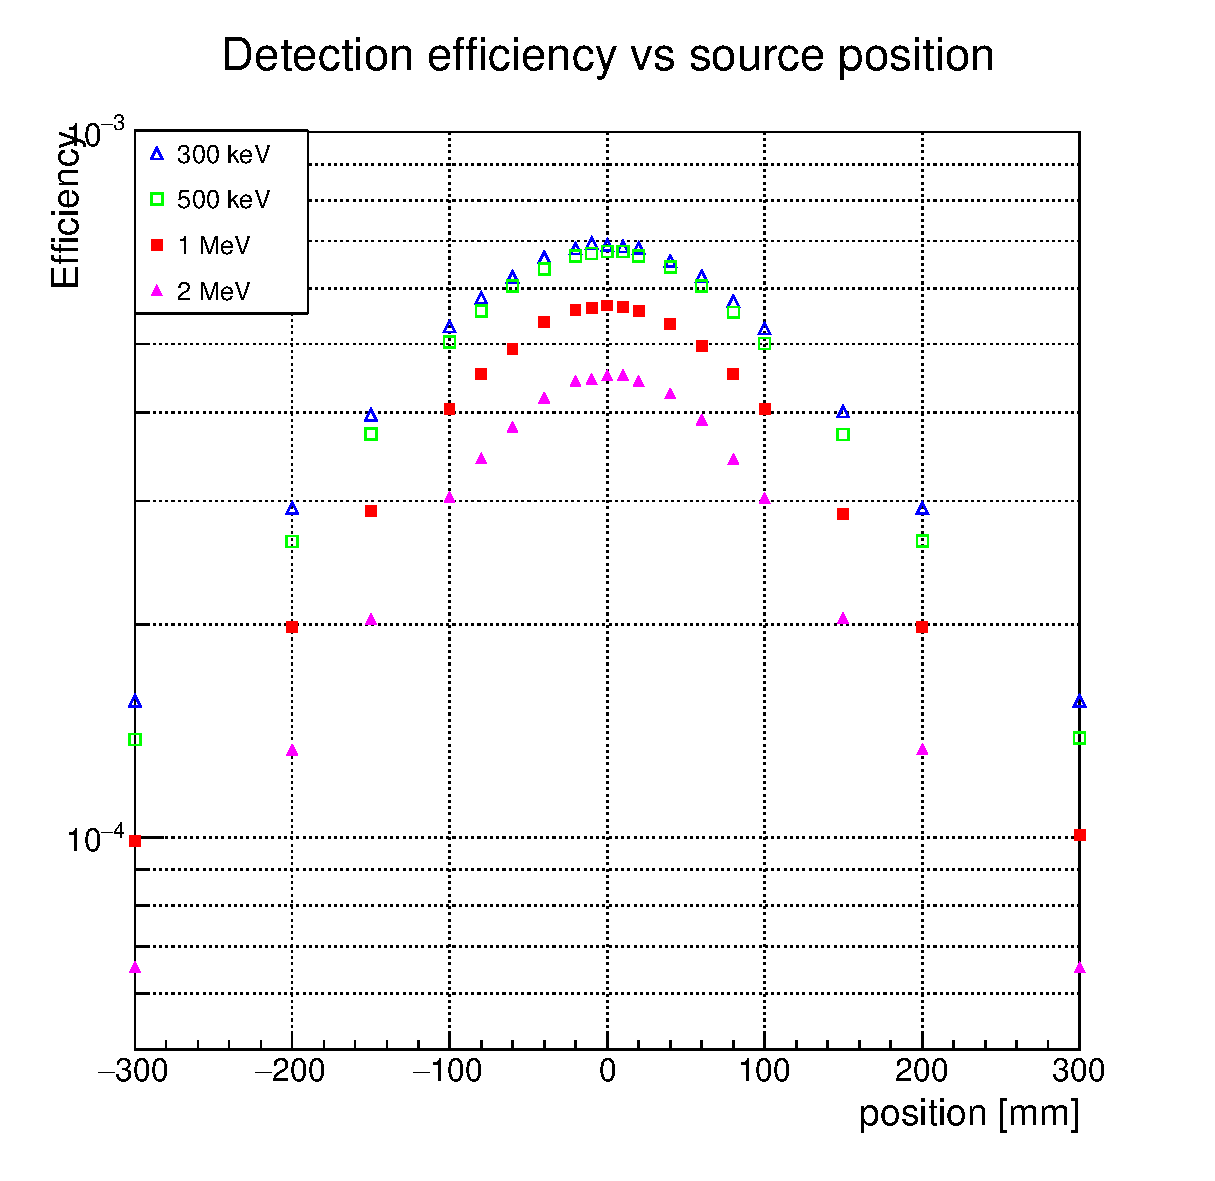
\includegraphics[width=0.7\textwidth]{./Figure/Efficiency/2017-06-26_Efficiency_CC_articles.eps}
	\end{figure}


\subsection{Beam intensity \newline}
Je traite les simulations pour une statistique de $10^{8}$ pour les protons et une statistique de $2\times10^{5}$ pour les ions carbone.\newline
J'assigne à chaque particule interagissant dans le diffuseur et l'absorbeur un numéro de paquet auquel elle est théoriquement rattachée au vu de la structure en temps choisie et de l'intensité du faisceau.
The modification of the beam intensity will change the number of particles included in a bunch. For instance, at the clinical intensity in protons, there is in average 217 protons in a bunch.



The beam intensity plays an important role for the Compton camera concerning its capability to distinct events in coincidence. In the simulation, the beam intensity is modeled by an average number of particles per bunch. The exact number of particles in each bunch is given by a random draw in a Poisson distribution, where the mean value is the beam intensity chosen. The range of intensities was chosen in order to cover almost all the possibilities: from a very low beam intensity to the clinical beam intensity. Therefore, for proton and carbon ion, the lowest beam intensity is set to 0.001 particles per bunch in average and for protons goes up to 217 protons per bunch when in case of carbon ion, it goes up to 70 particles per bunch. The coincidence yields are scaled per ion incidents and the beam intensity per average ions per bunch. The true coincidences represent a coincidence in the camera by the same gamma ray. The background corresponds to all the other coincidence types.


\begin{figure} [!h]
\caption{Coincidences yield for protons (a) and carbon ions (b) in function of the beam intensity. The intensity is given for a number of incident particles per bunch.  The distinction between the filled markers and the empty ones are that the time of flight discrimination is applied in the case of empty markers.}
\subfloat[]{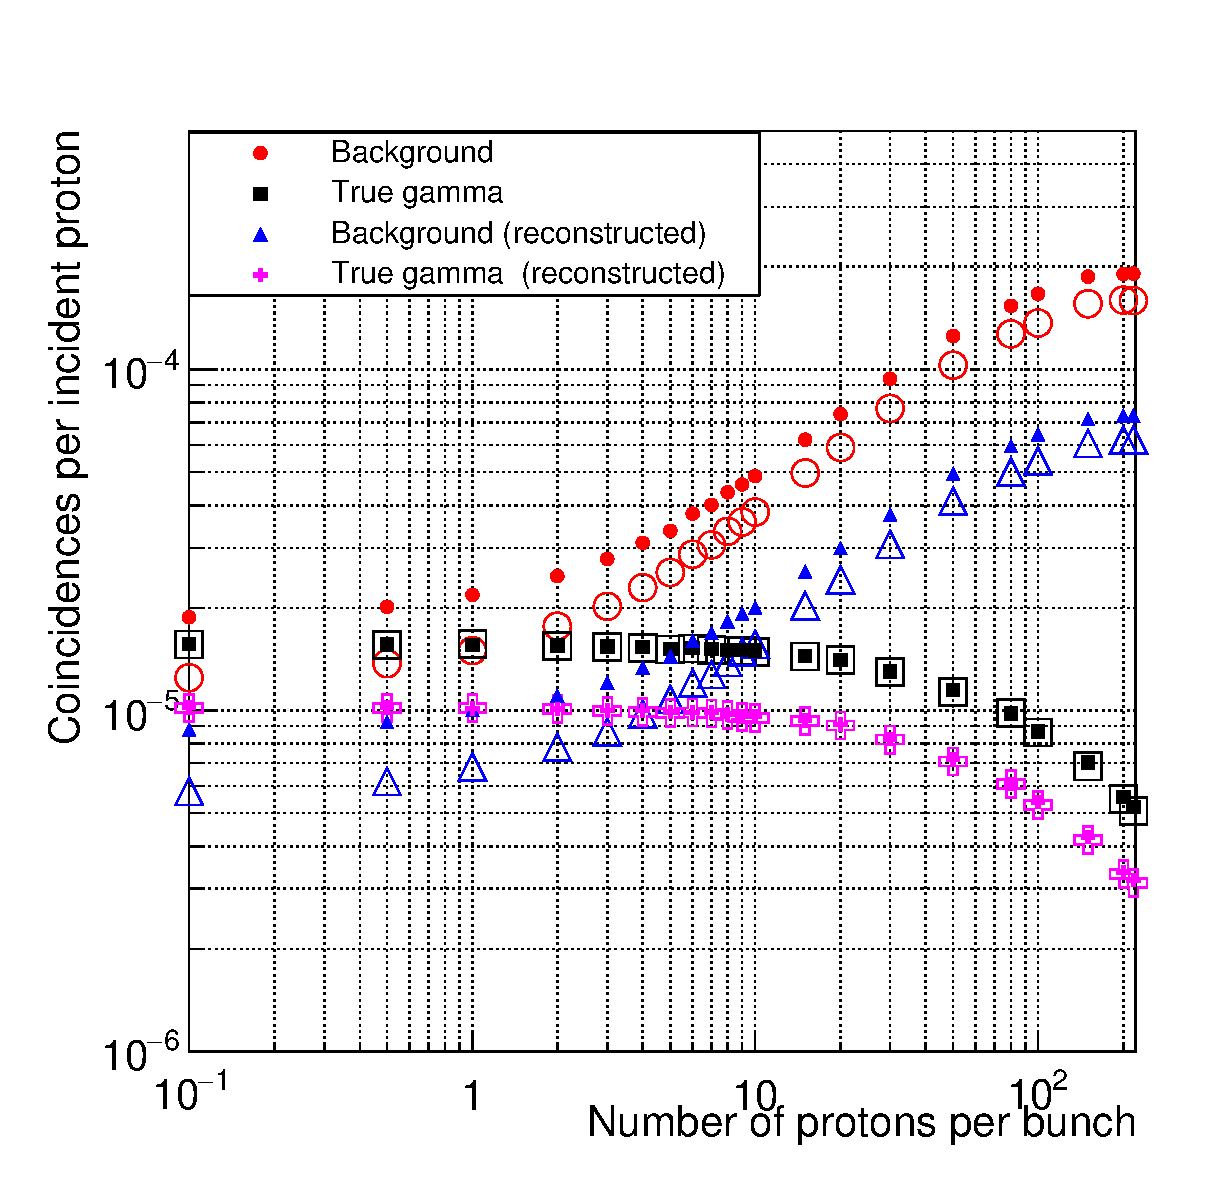
\includegraphics[width=0.5\textwidth]{./Figure/Beam_Intensity/2017_06_28_Taux_coincidences_variation_protons_New_design_4EntreesLegend_LogXLogY.eps}}
 \subfloat[]{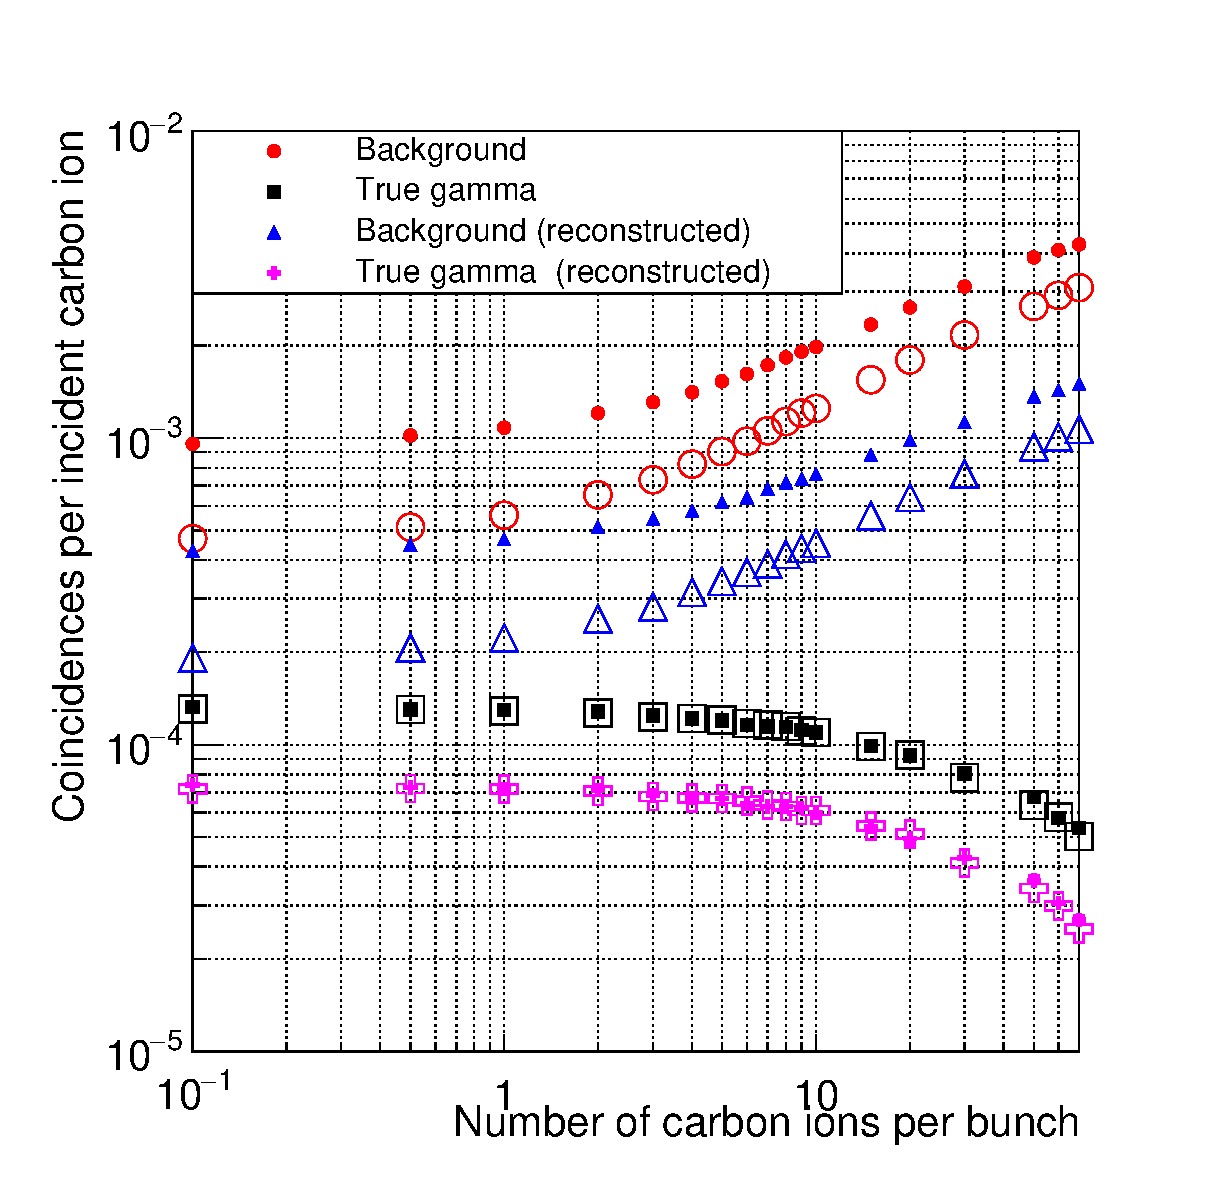
\includegraphics[width=0.5\textwidth]{./Figure/Beam_Intensity/2017_06_28_Taux_coincidences_variation_carbonIons_New_design_4EntreesLegend_LogXLogY.eps}}
  \label{fig:coincidences}
\end{figure}

\newpage
At the clinical beam intensity, the high background level is mainly due to the random coincidences. In fact, the probability to detect two radiation coming from two different incident particles increases with the number of incident particles per bunch. Another issue is the single rate of events detected by each detector at those high intensities. For instance, at the clinic beam intensity in proton therapy, the single rate on the absorber is around 300 MHz and on the first silicon layer it is around 20 MHz. The current electronic front end and acquisition system are not able to treat this amount of data coming from all the detectors. As a result, it appears that it is impossible to use the Compton camera at a clinical beam intensity for the treatment monitoring in ion therapy.\newline
Nevertheless, if the intensity decreases enough to avoid almost all the random coincidences, the monitoring seems more feasible. In addition, it can be supposed that the time of flight discrimination will improve the signal to the background ratio at low intensities by suppressing the coincidences induced by charged particles. Indeed, the charged particles are slower than gamma rays which move at the light speed.\newline

\subsection{Comparaison LM-MLEM vs Line cone reconstruction\newline}


\begin{figure} [!h]
\caption{Comparaison LM-MLEM vs Line cone reconstruction}
\subfloat[]{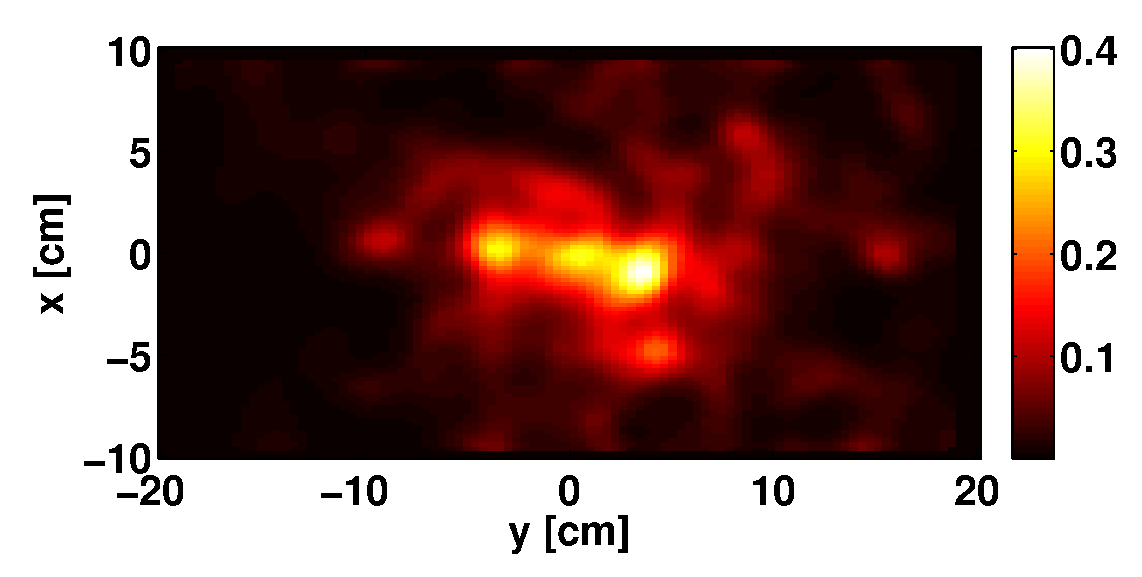
\includegraphics[width=0.5\textwidth]{./Figure/MLEM/2015_10_20_Volume_100x100x5_voxels_and_size_20x40x1_source_Proton160MeV_camera_50mm_stat_2175events_sans_MatriceSensibility_bordYplusmoins-3_bordXplusmoins-3_median_iteration_10.eps}}
 \subfloat[]{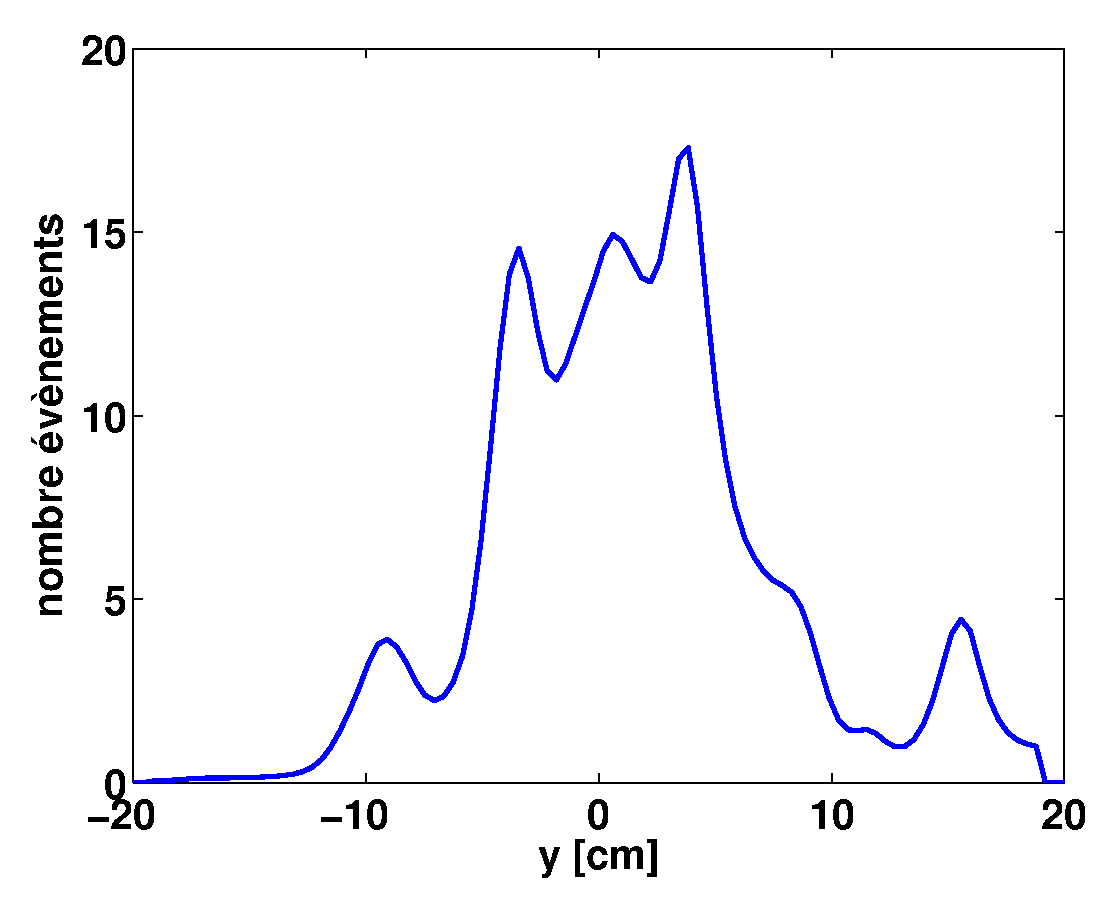
\includegraphics[width=0.5\textwidth]{./Figure/MLEM/2015_10_20_Volume_100x100x5_voxels_and_size_20x40x1_source_Proton160MeV_camera_50mm_stat_2175events_sans_MatriceSensibility_bordYplusmoins-3_bordXplusmoins-3_selectionX_20mm_Filtre_median_iteration_Profil_Y_iteration_10.eps}}\\
  \subfloat[]{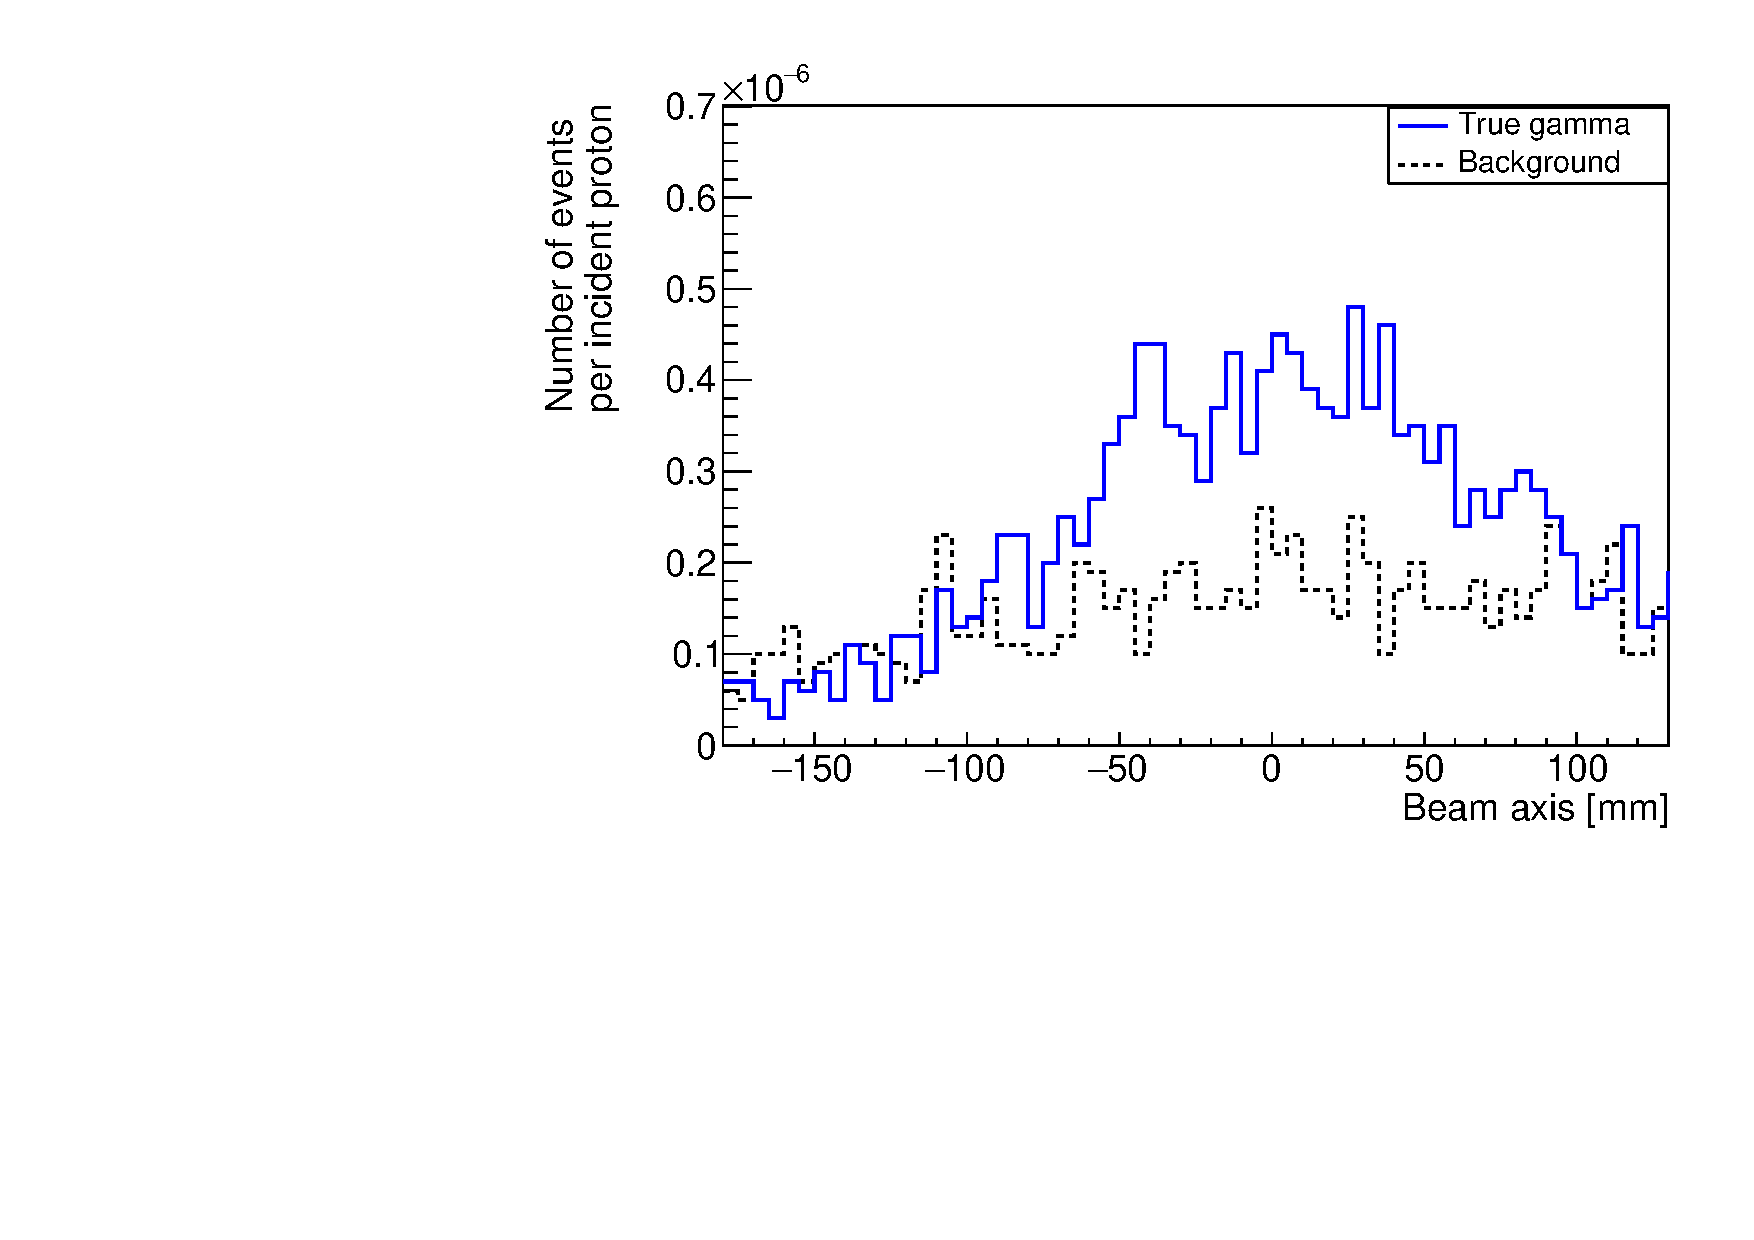
\includegraphics[width=0.5\textwidth]{./Figure/MLEM/2015_02_16_Reconstruction_coinc_160MeVProton_TOF_6ns_file0to100_zoom.pdf}}
  \label{fig:comparaison}
\end{figure}


\subsection{Compton camera precision\newline}

The information given by a control device as the Compton camera has to be viable and as precise as possible. In order to estimate the precision of the Compton camera, a method is used. 



\newpage
\section{Discussion}


\newpage
\ack

This work is supported by the FP7-ENVISION program WP3, the FP7-ENTERVISION program, the FP7- ULICE program, the ANR Gamhadron project, the Rhone-Alpes Regional Program for Hadrontherapy Research, the MI2B GDR and the LabEx PRIMES.\newline

\bibliographystyle{apalike}
\addcontentsline{toc}{part}{Bibliographie}
\bibliography{Biblio_13}



\end{document}

